\documentclass{scrreprt}

\usepackage{aligned-overset}
\usepackage{amsmath}
\usepackage{amssymb}
\usepackage{bm}
\usepackage[shortlabels]{enumitem}
\usepackage{hyperref}
\usepackage[utf8]{inputenc}
\usepackage{multicol}
\usepackage{mathtools}
\usepackage{physics}
\usepackage{struktex}
\usepackage{tabularx}
\usepackage{titling}
\usepackage{fancyhdr}
\usepackage{xfrac}
\usepackage{pgfplots}

\pgfplotsset{compat = newest}
\usetikzlibrary{intersections}
\usetikzlibrary{patterns}
\usetikzlibrary{positioning}
\usepgfplotslibrary{fillbetween}

\author{Karsten Lehmann}
\date{WiSe 2021/2022}
\title{Vorlesungsnotizen\\Algorithmen und Datenstrukturen}

\setlength{\headheight}{26pt}
\pagestyle{fancy}
\fancyhf{}
\lhead{\thetitle}
\rhead{\theauthor}
\lfoot{\thedate}
\rfoot{Seite \thepage}

\begin{document}
\paragraph{Der Weg vom Problem zum Programm}

\begin{center}
  \begin{tikzpicture}
    \node[draw, rectangle, rounded corners=3pt] at (2, 0) (problem) {Problem};
    \node[draw, rectangle, right=of problem, rounded corners=3pt] (problem_spec) {Problemspezifikation};
    \node[draw, rectangle, right=of problem_spec, rounded corners=3pt] (algo) {Algorithmus};
    \node[draw, rectangle, right=of algo, rounded corners=3pt] (prog) {Programm (in C)};
    \node[below = 0cm of problem_spec, blue] {formales Objekt};
    \draw[->] (0, 0) -- (problem) node[below left = 0.5cm and 1.7cm, rotate=90] {Problemformulierung};
    \draw[->] (problem) -- (problem_spec) node[below left = 0.5cm and 2.7cm, rotate=90] {Problemanalyse, -abstraktion};
    \draw[->] (problem_spec) -- (algo) node[below left = 0.5cm and 2cm, rotate=90] {Algorithmenentwurf};
    \draw[->] (algo) -- (prog) node[below left = 0.5cm and 2.5cm, rotate=90] {Programkonstruktion};
  \end{tikzpicture}
\end{center}

\textbf{Beispiel:} Das Problem besteht darin, die jüngste Person in einem Raum
zu ermitteln.
In der Problemanalyse wird das Problem mit wichtigen Fragen umrandet.
\begin{itemize}
\item Gibt es eine jüngste Person? (Existiert eine Lösung?)
\item Ist die Lösung (falls vorhanden) eindeutig?
\item Wie soll die Lösung denn aussehen?
\item Was passiert, wenn zwei Personen gleich alt sind?
\end{itemize}

Diese Fragen führen zu Abstraktionen.
Zum Beispiel wird jede Person durch eine natürliche Zahl $i$ repräsentiert.
Jede Person $i$ hat ein Alter $a_i$ (in Jahren).
Die Zahlen $a_1, \ldots, a_n$ werden als bekannt angenommen.
Die jüngste Person wird definiert als die Person $i$, für welche gilt:
für jede Person $j$ gilt $a_i \leq a_j$.
Falls zwei Personen $i$ und $j$ gleich alt sind, also $a_i = a_j$, dann wird die
erste Person mit dem Alter $a_i$ als Lösung bestimmt.

Aus diesen Abstraktionen folgt schließlich ein formales Objekt - nämlich die
Problemspezifikation:
\begin{itemize}
\item \emph{Gegeben} ist eine Folge $a_1, \ldots, a_n$ von natürlichen Zahlen.
\item \emph{Gesucht} ist der kleinste Index $i$ mit
  $a_i = \min\qty{a_1, \ldots, a_n}$.
\end{itemize}

Der Spezifikation folgt ein \textbf{Algorithmus}.
Ein \textbf{Algorithmus} ist eine (Rechen-)Vorschrift zur Lösung des Problems.
Dabei muss der Algorithmus so präzise formuliert werden, dass er maschinell
ausgeführt werden kann.
Der Algorithmus ist immer unabhängig von der verwendeten Programmiersprache.
Weiterhin muss der Algorithmus drei Eigenschaften erfüllen:
\begin{itemize}
\item \emph{Finitheit}: Der Algorithmus wird durch einen endlichen Text
  beschrieben.
\item \emph{Effektivität}: Der Algorithmus läuft in einzelnen, wohldefinierten
  Schritten ab.
\item \emph{Determiniertheit}: Der nächste Schritt ist immer eindeutig
  festgelegt.
\item \emph{Terminiertheit}: Unabhängig von der Eingabe kommt der Algorithmus
  in endlich vielen Schritten zum Ende.
\end{itemize}

\begin{struktogramm}(120, 70)
  \assign{Eingabe : Folge $a_1, \ldots, a_n$ von natürlichen Zahlen}
  \assign{$j = 1$}
  \assign{$x = a_j$}
  \assign{$i = 2$}
  \while[1]{Solange $i \leq n$}
    \ifthenelse{3}{3} {$a_i < x$} {Ja}{Nein}
      \assign{$j = i$}
      \assign{$x = a_j$}
      \change
    \ifend
    \assign{$i = i + 1$}
  \whileend
  \assign{Ausgabe: $j$ als Ergebnis}
\end{struktogramm}

Schließlich folgen noch Fragen zu der zu verwendenden Programmiersprache,
der Eingabe der Daten, den verwendeten Datenstrukturen und der Art, in der das
Ergebnis ausgegeben wird.

\paragraph{Sprachen} werden Unterschieden in Objektsprachen (zum Beispiel
Deutsch) und Metasprachen (zum Beispiel die Grammatik der Deutschen Sprache).
Programmiersprachen sind Objektsprachen.
Die Metasprachen für die Programmiersprachen sind Syntaxdiagramme
und EBNF (Erweiterte Backus-Naur-Form).
Auch \emph{formale Sprachen} sind Objektsprachen und lassen sich durch
Kontextfreie Grammatik (Typ-2-Grammatik) oder Kellerautomaten beschreiben.

Zur Beschreibung von formalen Sprachen wird ein Symbolvorat benötigt.
Dieser Symbolvorat wird \emph{Alphabet} genannt.
Ein Alphabet ist eine nichtleere, endliche Menge von Symbolen.

Sei nun $\Sigma$ ein Alphabet, dann bezeichnet ein
\emph{Wort über $\Sigma$} eine endliche Folge von Symbolen aus $\Sigma$.

Ein besonderes Wort ist das Wort mit der Länge $0$, beschrieben als
$\epsilon$.

Die \emph{Menge aller Wörter} über dem Alphabet $\Sigma$ wird mit $\Sigma^*$
beschrieben.

Schließlich bezeichnet eine \emph{formale Sprache $L$ über $\Sigma$} die Menge
von Wörtern über $\Sigma$, dass heißt $L \in P(\Sigma^*)$.

\end{document}